 \documentclass[12pt]{article}
\usepackage[paper=a4paper, bottom=32mm, footskip=-15mm, headheight=5mm]{geometry}
\usepackage[utf8]{inputenc}
\usepackage{graphicx}
\graphicspath{ {./figures/} }
\usepackage{amsmath} 
\usepackage{hyperref}
\usepackage{fancyhdr}
\usepackage{lipsum}
\usepackage{xcolor}
\usepackage{tikz}
\usepackage[shortlabels]{enumitem}
\PassOptionsToPackage{hyphens}{url}\usepackage{hyperref}

\begin{document}

\begin{titlepage}
    \begin{center}
        \begin{figure}[t]
            \centering
            \includegraphics[width=0.95\textwidth]{figures/metu.png}
        \end{figure}
        \Large{\textbf{EE463 | Static Power Conversion - I}} \\
        \Huge{\textbf{Hardware Project Report}} \\
        \Large{Happy EE Friends} \\
        \vspace*{15 mm} 
        \large
        Arda KASIM - 2232197 \\
        Atilla Can AYDEMİR - 2374510 \\
        Eminalp KOYUNCU - 2307882 \\
        \vspace*{\fill}
        \begin{figure}[h]
          \centering
          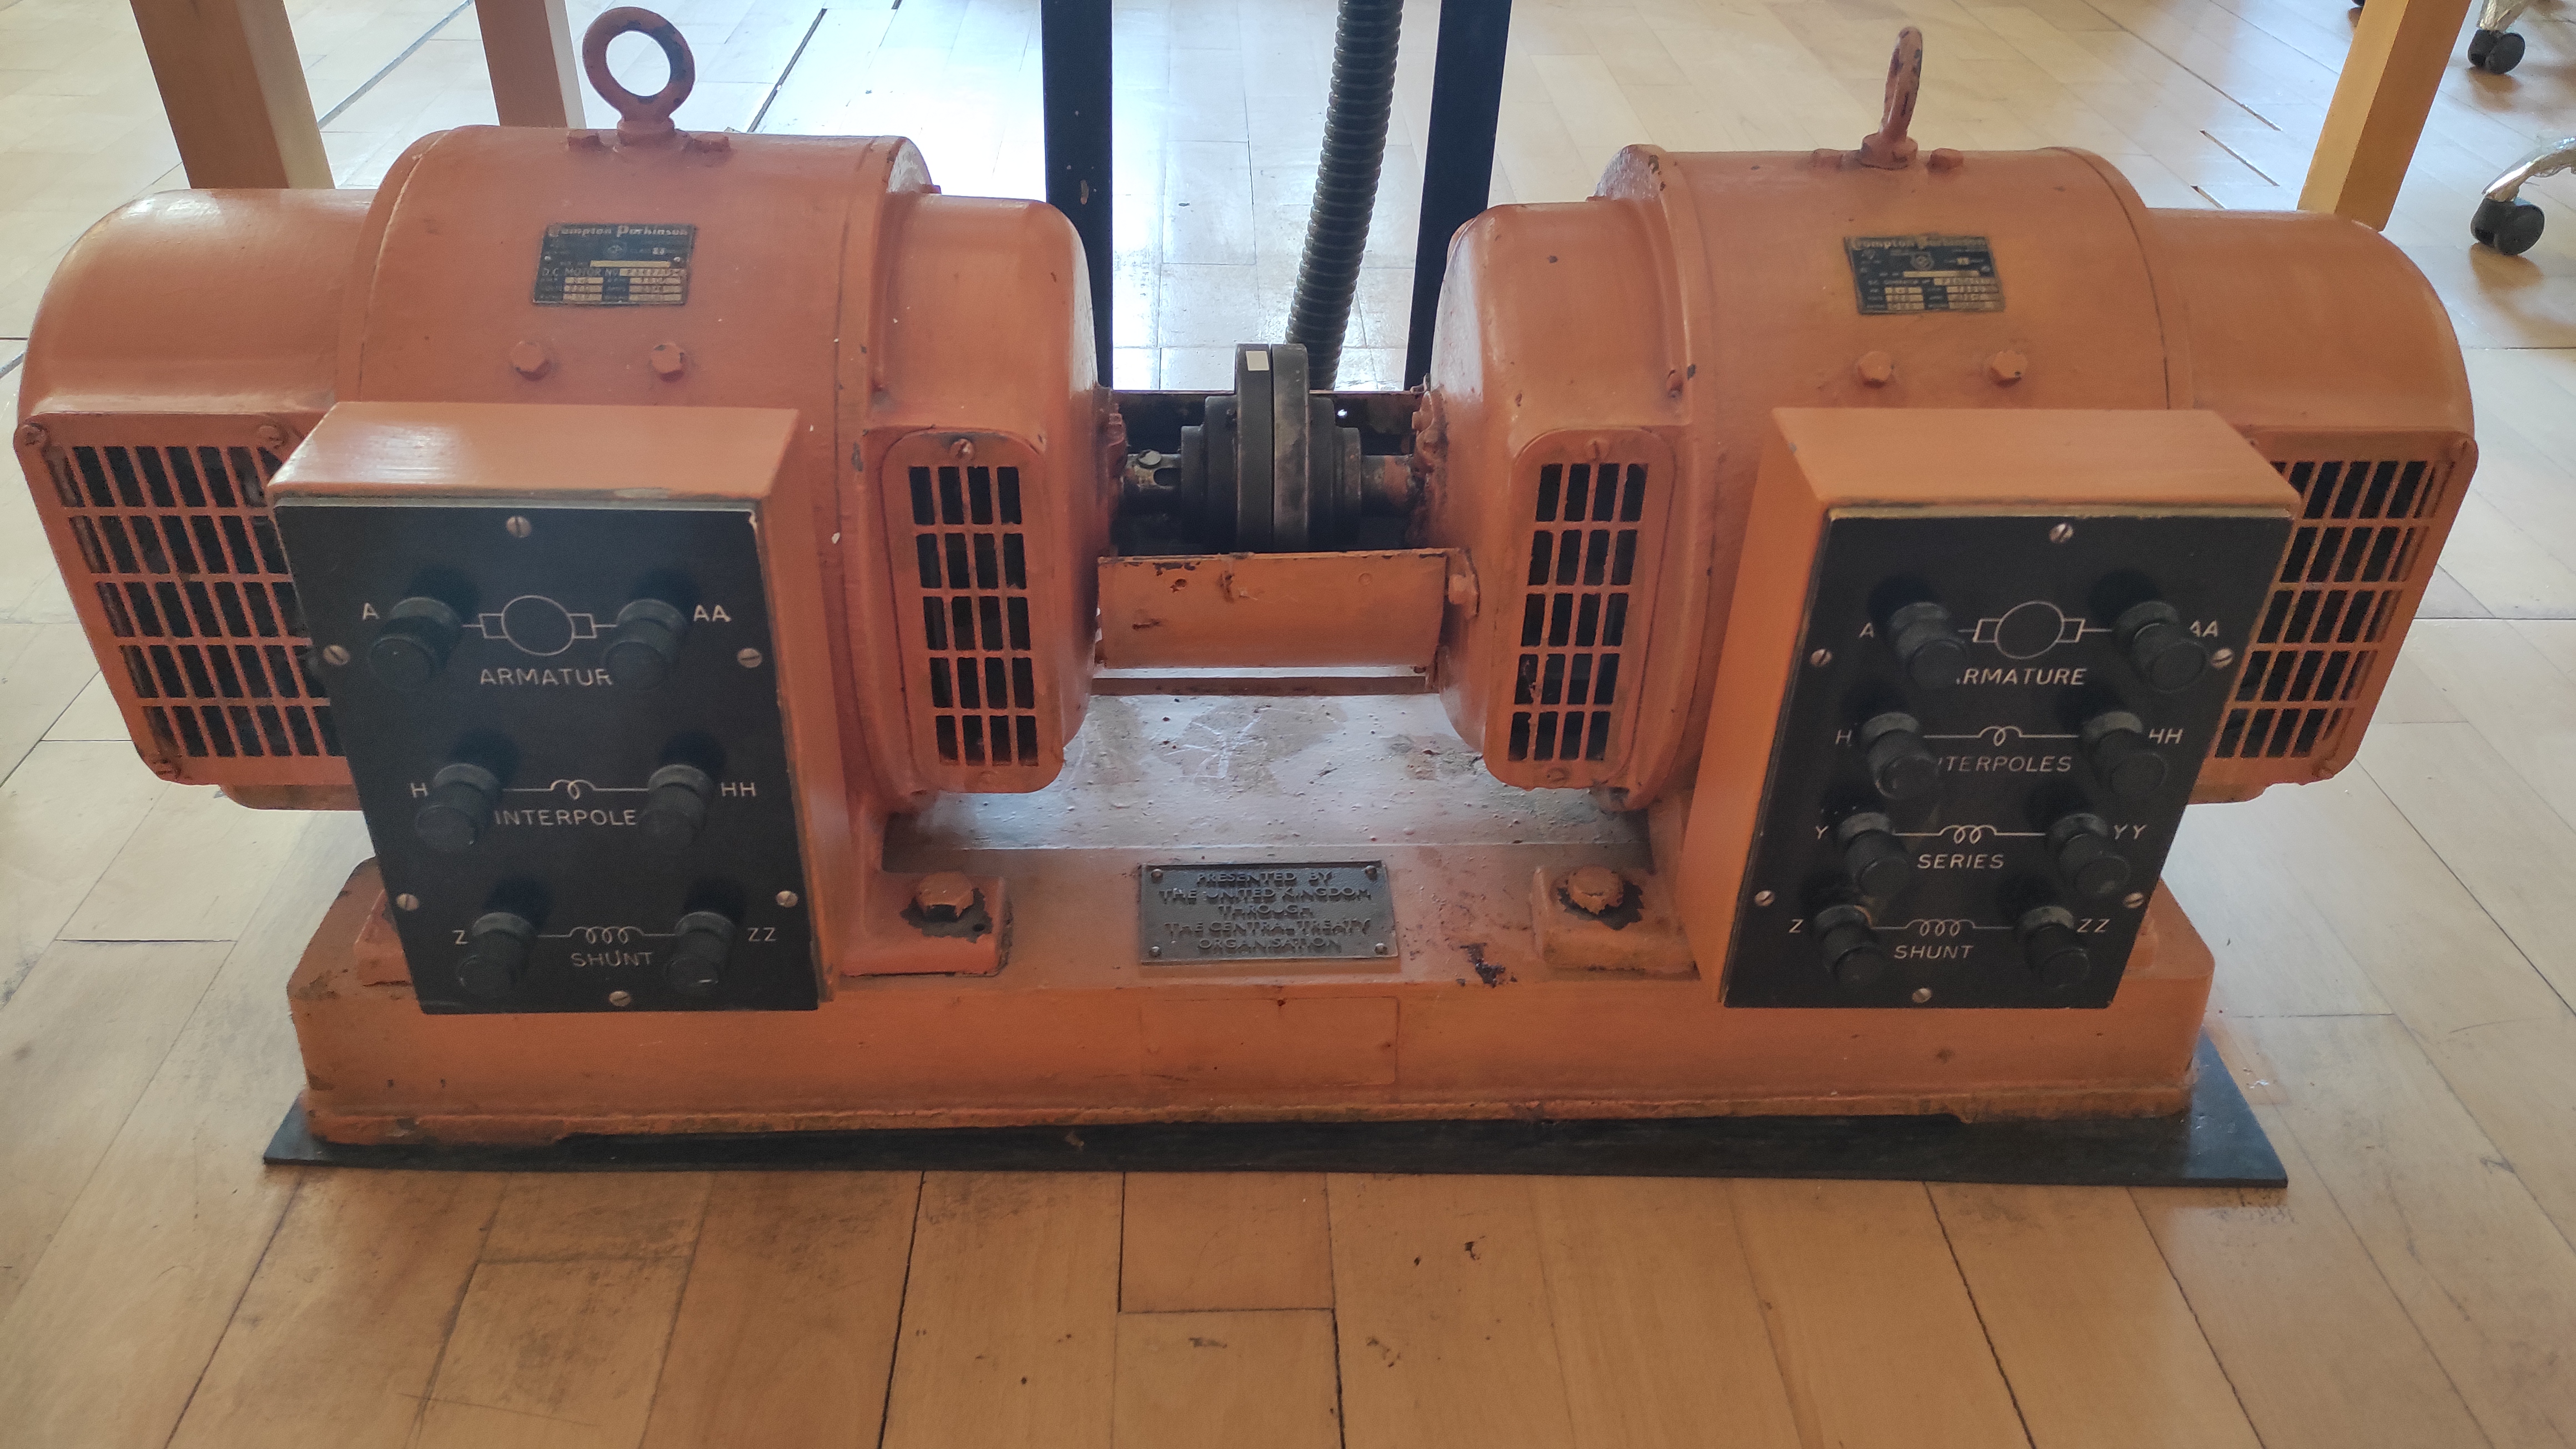
\includegraphics[width=0.95\textwidth]{figures/motor-set.jpg}
        \end{figure}
        \vspace*{\fill}
           January 2023
        \end{center}
\end{titlepage}

\pagestyle{fancy}
\fancyhead{}
\fancyhead[L]{\textbf{Hardware Project Report}}
\fancyhead[R]{\textbf{Happy EE Friends}}
\section{\Large Introduction}
\raggedright
In this report, the design process of the AC-DC converter is analyzed. The simulations and the data obtained while implementing and demonstrating the hardware project are shown in the report with explanations on the component selection are included. In the project, we have used rectifiers, buck converter, gate drivers, capacitances, and isolators. The problems encountered in the demonstration of the project are discussed and possible explanations for the failures of the hardware project are analyzed. 
\section{\Large Topology Discussion}
\subsection{AC/DC Conversion}
When all the topologies are compared, 3-phase full-bridge diode rectifier topology is selected. The high output voltage ripple and comparatively lower output voltage value of the single-phase rectifiers are the reasons why single phase rectifiers are not selected. Also, in the single-phase rectifiers there are higher order harmonics and as a result the THD of the rectifier is greater, while the 3-phase rectifiers eliminate the third order harmonics completely and the THD is lower than the single-phase rectifiers.  The edge of the 3-phase full-bridge diode rectifier over the thyristor rectifier is simplicity and easier control. Each thyristor would need a gate signal, which would complicate the system by both cabling and control standpoint. The relative simplicity and superior qualities of the 3-phase full-bridge rectifier topology were the main reasons in the selection of it as the AC-DC rectifier topology. To realize this topology, 6 diodes are needed, and these diodes are selected according to the simulations, which will be discussed in the component selections and simulations parts.
\subsection{DC/DC Conversion}
After selecting 3-phase full-bridge rectifier topology, a need for DC/DC conversion has come up. As the variac voltage was set to a fixed level, the average DC voltage would be a constant level at the output of the diode rectifier. This meant that achieving a soft-start would be impossible and the converter would blow up immediately when powered up. We have decided to implement a switching mode converter after the rectifier to gain control over the voltage level. We have done this using a buck converter as our DC average voltage could be achieved at a higher level than motor ratings and buck converter would be easy to implement.
\section{\Large Design}
\subsection{Pre-Design Considerations}
After finalizing our choices we started our design based as a 3-phase full-bridge diode rectifier + buck converter. We also discussed about the extra features we were planning to implement for bonuses and took according design steps. These extra features were
\begin{itemize}
    \item Tea Bonus
    \item PCB Bonus
    \item Industrial Design Bonus
    \item Single Supply Bonus
    \item Closed-loop Current Control Bonus (EE407)
    \item Closed-loop Speed Control Bonus (EE407)
\end{itemize}
We decided to use an Arduino for our logical operations therefore there was a need to implement an extra conversion to lower voltage levels around 9V to power it up so that we could operate with single AC supply. Also, we have drawn a PCB layout to provide a neat design. Component selections was done considering 2kW rated load conditions.
\subsection{Design Approach}
Our motor is rated at 220V average, which must be divided by our steady state duty cycle so that we can find the maximum voltage that the components will be exposed to. Considering a general case for D = 0.5, we limited our search within voltages higher than 440v. Our current rating will be around 12A considering tea bonus and losses. \smallskip \\
We started our design from 3-phase full-bridge diode rectifier where we initially searched for single diodes whose ratings are within our operating point. It was revealed shortly after that purchasing a package which has all 6 diodes would be both cheaper and more efficient. \smallskip \\
During the design of buck converter, we decided to omit the inductor; as the motor itself acts as a high inductive load. Also, we stayed within limits while picking components, except for one (unfortunately revealed during demonstration), and finalized our selection. \smallskip \\
After the components were chosen, we started drawing it on PCB immediately; without any prototype attempts. This was due to lack of time, and also due to our trust at PCB being more stable than any other prototyping methods.
\subsection{Arduino Supply Circuitry}
We have designed another AC/DC converter circuitry for Ardiuno voltage supply with a transformer and linear regulator. The transformer had a 230/12 turns ratio which lowered a grid level AC voltage to 12V RMS. A single phase full-bridge diode rectifier was connected at the secondary side of the transformer to rectify the AC voltage to DC. This voltage then filtered with a 1000\begin{math} \mu F \end{math} capacitor and supplied to a linear dropout (LDO) regulator with a fixed 9V output voltage rating with up to 1.5A current rating. The current rating was selected as high as possible in order to supply the gate driver with the output of LDO as well.
\subsection{PCB Design}
We have prepared schematics and layout using KiCad as the software offered a fast learning curve thanks to its simple interface. KiCad also offers a considerably large library for components together with baselines for almost all IC packages which can be easily adapted for any component. \\
\subsection{Design Errors}
\subsubsection{PCB Clearance}
When the circuit was given input voltage for the first time, current has jumped and exploded two of the input paths of the 3-phase full-bridge rectifier. After the malfunction, it is analyzed that either the lack of clearance of those paths provided a jumping opportunity for the current, or the soldering was not done properly such that current has jumped between the paths. This meant high amounts of voltage difference between two points, which almost don’t have any resistance. This high current exploded two of the input paths of the rectifier.
\subsubsection{Arduino Supply Circuitry}
Although the circuitry worked as intended, there was a fundamental error with the design that it required 100\% variac voltage to operate. Firstly, 100\% variac voltage would end up around 540V at the output of the diode bridge, leading a very difficult operation of buck converter. Secondly, in order to control the gate signal of the buck converter we needed to power up Arduino first. However; as both the main converter and low voltage converter operated simultaneously, there was a need to provide AC voltage to both of them at the same time. It was reveal experimentally that, the voltage that could power up the Arduino was around 130VAC. Therefore the circuit wouldn't operate below 130V, and wouldn't operate as intended around 130V as the LDO couldn't supply 9V at those levels. This led to us giving up on single supply bonus.
\subsubsection{MOSFET PCB Footprint}
There was a minor error in the MOSFET footprint where we had drawn it as D-G-S configuration. The correct order was G-D-S and we fixed this by cutting the drain pin and soldered it to its correct position with a cable. We connected the gate pin with a slight bent to achieve a lower parasitic inductance compared to connecting with a cable.
\subsection{Failures at Implementation}
Throughout the implementation of the project, several different errors were encountered. Although most of them were identified and corrected, at both project demonstrations some new problems have occurred which resulted in the failure of the hardware project. Regardless, in this report these new errors have been analyzed and possible solutions to them are proposed.
\subsubsection{Misplaced Components}
\subsubsection*{Freewheeling Diode}
While soldering the components on PCB, the freewheeling diode was soldered in the opposite direction. This would cause short circuit on the circuit when the switch was turned on, so X volts of potential would flow on a path with minimum resistance. This high amount of current would be too much for the components of the system and the path of current on the PCB would explode, together with the MOSFET and freewheeling diode. After PCB was severely damaged, the decision to transfer the project to soldering board was taken.
\subsubsection*{Capacitor}
The DC motor we were aiming to drive can be modelled as a high inductive load. In the first proposed topology, the capacitor was placed after the buck converter as parallel to the DC motor. However, this would not be meaningful because the aim of putting a capacitor in the system was to increase the output voltage characteristics and make it smoother. This output voltage would then be transmitted to the buck converter and this steady voltage would be critical to eliminate voltage differences between each switch, which would amount to high current values at each switching. For this purpose, the capacitor was moved to the output of the rectifier such that the output voltage would be smoother, and ripple would be minimal.
\subsubsection{Soft Start Problem}
At first demonstration, the soft starting was aimed to be done by adjusting a pot by hand. However, this method proved to be unhealthy, as trying to soft start the DC motor manually is prone to human error. In the demonstration, pot was adjusted faster than it’s optimum rate, so a huge inrush current traversed the system and as a result two of the three fuses and MOSFET blew up. After the identification of this problem, a soft starting code was implemented into the Arduino such that there would be no human element in the soft starting. An optimal soft starting would mean no inrush current to disrupt the system. Indeed, in the final demonstration soft starting would not be a problem as the DC motor would start to run without any problem at low voltages.
\subsubsection{Wrong Component Selection}
The trials of the system were made at low voltage to understand whether the system would work at low voltages or not. It was concluded that with R load and RL load the system would work however high voltage was never tested. When high voltage was applied in the demonstration, the diode exploded and the system stopped working. Analysis of the system after the demonstration proved that 300V rating of the freewheeling diode was not sufficient for the operation and thus the system malfunctioned. This was the final error. Given that the system would manage to start the motor and run at low voltages without any problem, it is concluded that the voltage rating of the freewheeling diode was the only error remaining in the system and only possible future malfunction could be caused by thermal properties.
\subsubsection{Control Loops}
Due to insufficient time, we failed to implement the control loops to the system before the demonstration day. If we were able to implement them on time, the spark during the demonstration would not occur as we would have a current limiter integrated.
\section{Component List and Cost Analysis}
The components that were mounted on the prototype board with their costs are listed below. \\
\begin{tabular}{|c|c|c|c|}
    \hline
    \textbf{Component} & \textbf{\textbf{Description}} & \textbf{Ratings} & \textbf{Price (\$)} \\ \hline
    GUO40-12NO1 & 3-Phase Diode Bridge & 1200V-40A & \$12.37 \\ \hline
    IXGH24N60C4D1 & IGBT & 1200V-40A & \$4.17 \\ \hline
    DSEI30-06A & Diode & 1200V-40A & \$3.51 \\ \hline
    \begin{math} 330 \mu F \end{math} & Capacitor & 400V & \$2.61 \\ \hline
    TLP250 & Optocoupler & 35V-2A & \$1.68 \\ \hline
    IC-7809 & LDO & 9V-1.5A & \$0.32\\ \hline
    Arduino Nano & Microcontroller & 9V-2A & \$9.20 \\ \hline
    Prototype Board & - & - & \$2.38 \\ \hline
    Heatsink & for Diode Bridge & - & \$2.03 \\ \hline
    Heatsinks & for IGBT and Diode & - & \$0.5 \\ \hline
    Passives & for logic level components & R\&C & \$1.00 \\ \hline
    \textbf{Grand Total:} & & & \$39.77 \\ \hline
\end{tabular} \bigskip \\
Due to several faults, we have destroyed many components. The cost of those components are given in a seperate table.
\begin{tabular}{|c|c|c|c|}
    \hline
    \textbf{Component} & \textbf{Description} & \textbf{Fault Reason} & \textbf{Price (\$)}  \\ \hline
    ESAF92-03R & Diode & Misplacing &  \$1.44 \\ \hline
    PJZ22NA50A & MOSFET & Misplaced Diode & \$2.46 \\ \hline
    PCB & - & Misplaced Diode & \$21.27 \\ \hline
    GUO40-12NO1 & 3-Phase Diode Bridge & Misplaced Diode & \$12.37 \\ \hline
    ESAF92-03R & Diode & Voltage Rating &  \$1.44 \\ \hline
    IXGH24N60C4D1 & IGBT & Diode Spark & \$2.46 \\ \hline
    TLP250 & Optocoupler & Diode Spark & \$1.68 \\ \hline
    Arduino Nano & Microcontroller & Unknown & \$9.20 \\ \hline
    Arduino Nano & Microcontroller & Unknown & \$9.20 \\ \hline
    \textbf{Grand Total:} & & & \$61.52 \\ \hline
\end{tabular}
\section{\Large References}
\begin{itemize}
    \item \url{https://keysan.me} 
    \item Kim, S. H. (2017). Electric motor control: DC, AC, and BLDC motors. Elsevier.
\end{itemize}
\end{document}




